%! TeX program = xelatex

\documentclass[12pt, a4paper]{article}
\usepackage{cmap}
\usepackage[fontsize=12pt]{scrextend}
\usepackage[T2A]{fontenc}
\usepackage[utf8]{inputenc}
\usepackage[english,russian]{babel}
\usepackage{amsmath,amsfonts,amssymb,amsthm,mathtools}
\usepackage[left=20mm, top=20mm, right=20mm, bottom=20mm, nohead, footskip=1cm]{geometry}
\usepackage{multirow}
\usepackage{array}
\usepackage{multicol}
\usepackage{graphicx}
\usepackage{wrapfig}
\usepackage{indentfirst}
\usepackage{enumitem}

\usepackage{polyglossia}
\usepackage{titlesec}
\usepackage{sectsty}
\usepackage{setspace}
\usepackage{fontspec}
\defaultfontfeatures{Mapping=tex-text}

\usepackage{fancyvrb}
\fvset{tabsize=4}

\usepackage{lipsum}
\usepackage{tocloft}
\usepackage[dvipsnames]{xcolor}

\usepackage{caption}
%\captionsetup{labelfont=it, textfont=it}
%\captionsetup[figure]{name=Схема}

\usepackage{hyperref}

\hypersetup{
    colorlinks=false,
    linktoc=all
}
\urlstyle{same}

\setmainlanguage{english}
\setotherlanguage{russian}
\setkeys{russian}{babelshorthands=true}
\setmainfont{Times New Roman}
\newfontfamily\cyrillicfont{Times New Roman}
\setmonofont{FreeMono}
%\let\cyrillicfonttt\ttfamily
%\onehalfspacing

%\allsectionsfont{\centering}
\renewcommand{\cftsecleader}{\cftdotfill{\cftdotsep}}

%======================================SECTIONING=========================================
%\makeatletter
%\renewcommand*\l@section{\@dottedtocline{1}{1.5em}{2.3em}}
%\makeatother
%======================================SECTIONING=========================================

\pretolerance=6000
\tolerance=3000
\emergencystretch=4pt

\setlength\intextsep{10pt}

\graphicspath{{./visuals/}}
\setlength{\parskip}{0.3125cm}
\setlength{\parindent}{1.25cm}
\setlength{\columnsep}{1cm}
\author{Grigoryev Mikhail}
\title{Algs lab}

\begin{document}

\thispagestyle{empty}

\vspace{30mm}

\begin{center}
FEDERAL STATE AUTONOMOUS EDUCATIONAL INSTITUTION \\
OF HIGHER EDUCATION \\
ITMO UNIVERSITY

\vspace{40mm}

{\large \textbf{Report \\
on the practical task No. 7 \\
"Algorithms on graphs. Tools for network analysis."}}
\end{center}

\vspace{15mm}

\begin{flushright}
{\large Performed by \\
\textit{Mikhail Grigoryev (370852) \\
Semenova Valeria (370061) \\
Academic group J4133c \\}
Accepted by \\
Dr Petr Chunaev}
\end{flushright}

\vspace{80mm}

\begin{center}
St. Petersburg \\
2022
\end{center}

\newpage

\section*{Goal}
\addcontentsline{toc}{section}{Goal}

The use of the network analysis software Gephi.

\section*{Formulation of the problem}
\addcontentsline{toc}{section}{Formulation of the problem}

\begin{enumerate}
	\item Download and install Gephi.
	\item Choose a network dataset from \url{https://snap.stanford.edu/data/} with number of nodes at most 10000. You are free to choose the network nature and type (un/weighted, un/directed).
	\item Change the format of the dataset for that accepted by Gephi (.csv, .xls, .edges, etc.), if necessary.
	\item Upload and process the dataset in Gephi. Check if the parameters of import and data are correct.
	\item Obtain a graph layout of at least two different types.
	\item Calculate available network measures in Statistics provided by Gephi.
	\item Analyze the results for the network chosen.
\end{enumerate}

\section*{Brief theoretical part}
\addcontentsline{toc}{section}{Brief theoretical part}

Gephi is an open-source network analysis and visualization software package written in Java. It widely used both in academia and journalism as well as digital humanities such as history, political sciences and literature.

It was originally developed in the University of Technology of Compi{\`e}gne in France, then was noticed by Google. In 2010 a non-profit organization called Gephi Consortium was formed for further development of the package.

\section*{Results}
\addcontentsline{toc}{section}{Results}

\textbf{Steps 1-2.} Gephi was installed, then, from the stanford library a social network of LastFM users collected from the public API in March 2020 was selected. Nodes are LastFM users from Asian countries and edges are mutual follower relationships between them. The vertex features are extracted based on the artists liked by the users. The task related to the graph is multinomial node classification -- one has to predict the location of users. This target feature was derived from the country field for each user. Network statistics (graph is unweighted and undirected):
\begin{center}
\begin{tabular}{cc}
	\hline
	Parameter & Value \\ \hline
	Nodes & 7 624 \\
	Edges & 27 806 \\
	Density & 0.0009 \\
	Transitivity & 0.1787 \\ \hline
\end{tabular}
\end{center}

\newpage

\textbf{Steps 3-4.} The initial dataset was in \texttt{.csv} format supported by Gephi. Import parameters were checked on import:
\begin{figure}[!h]
\centering
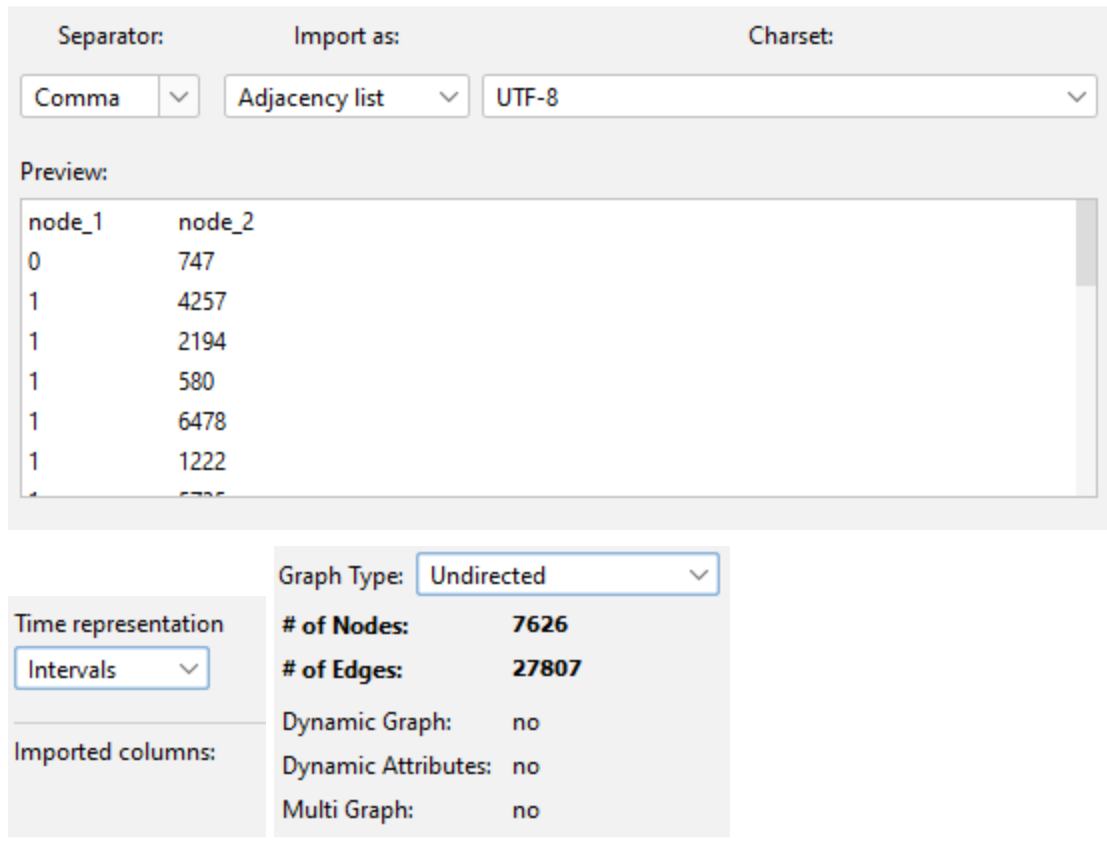
\includegraphics[width=0.6\textwidth]{s4p1.png}
\caption{Import parameters.}
\end{figure}

\textbf{Step 5.} Two layout types were used -- OpenOrd and YifanHu.

\begin{figure}[!h]
\centering
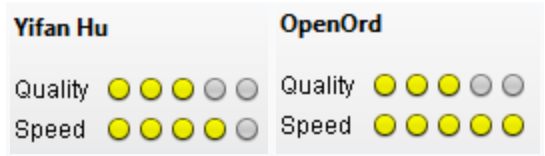
\includegraphics[width=0.4\textwidth]{s5p1.png}
\caption{Visualization type evaluations from Gephi.}
\end{figure}
\textit{OpenOrd} is Force-Directed layout algorithm for real-world large-scale undirected graphs. It can scale to over 1 million nodes, making it ideal for large graphs. However, small graphs (hundreds or less) do not always end up looking good. This algorithm expects undirected weighted graphs and aims to better distinguish clusters.
\begin{figure}[!h]
\centering
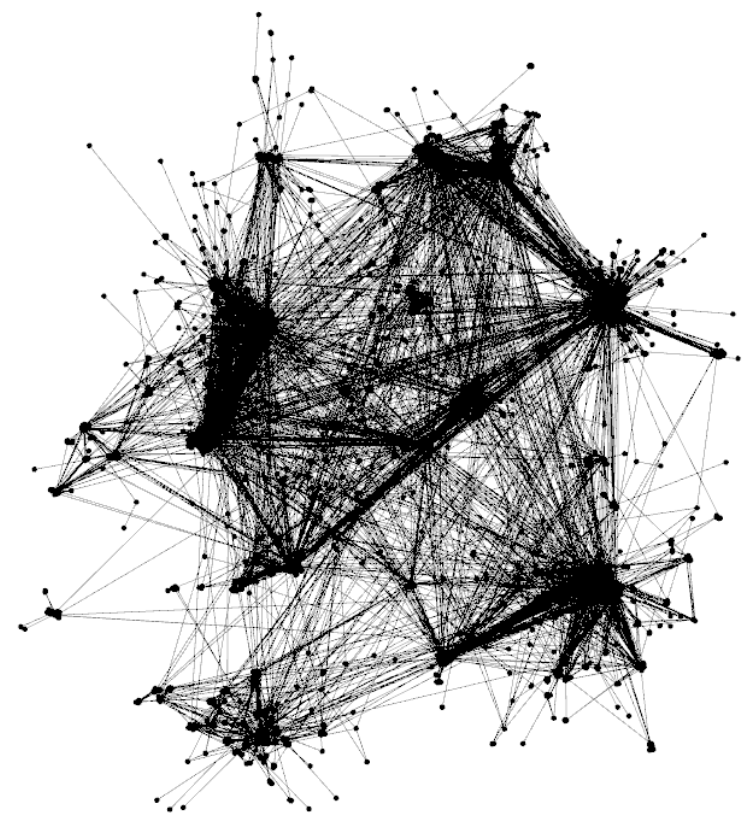
\includegraphics[width=0.4\textwidth]{s5p2.png} \hspace{5mm}
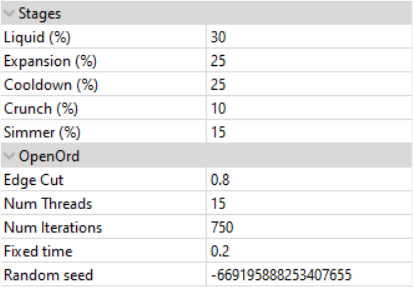
\includegraphics[width=0.45\textwidth]{s5p3.png}
\caption{OpenOrd layout visualization and preset.}
\end{figure}

\noindent
\textit{Yifan Hu} is the original Yifan Hu's attraction-repulsion model. It reduces the computational cost by restricting force calculation to the neighborhood. The algorithm stops itself, as it has an adaptive cooling scheme.
\begin{figure}[!h]
\centering
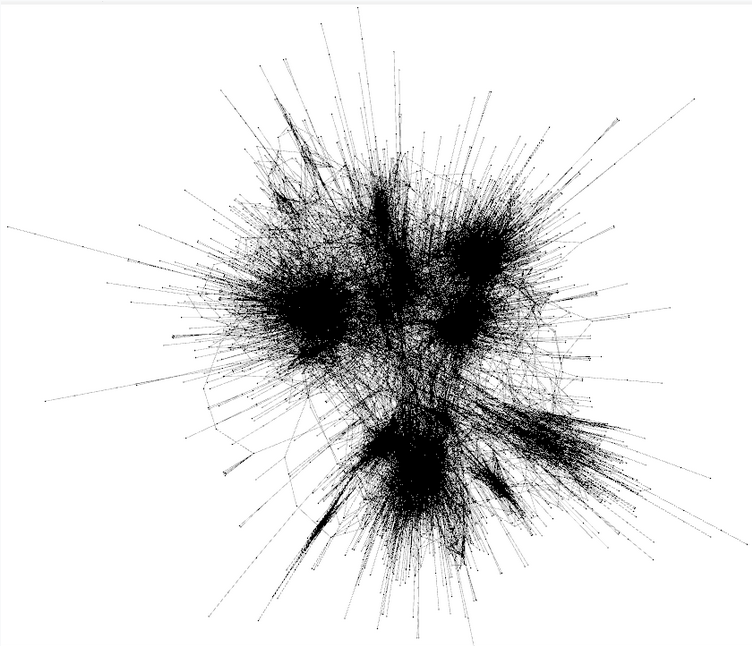
\includegraphics[width=0.45\textwidth]{s5p4.png}
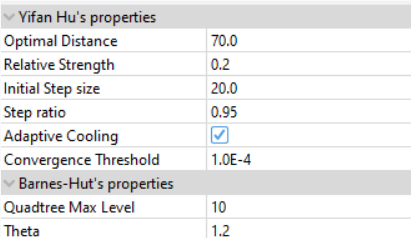
\includegraphics[width=0.45\textwidth]{s5p5.png}
\caption{YifanHu layout visualization and preset.}
\end{figure}

\textbf{Step 6.} Available network measures were taken from Gephi's Statistics. Reports are presented in the figures below.
\begin{figure}[!h]
\centering
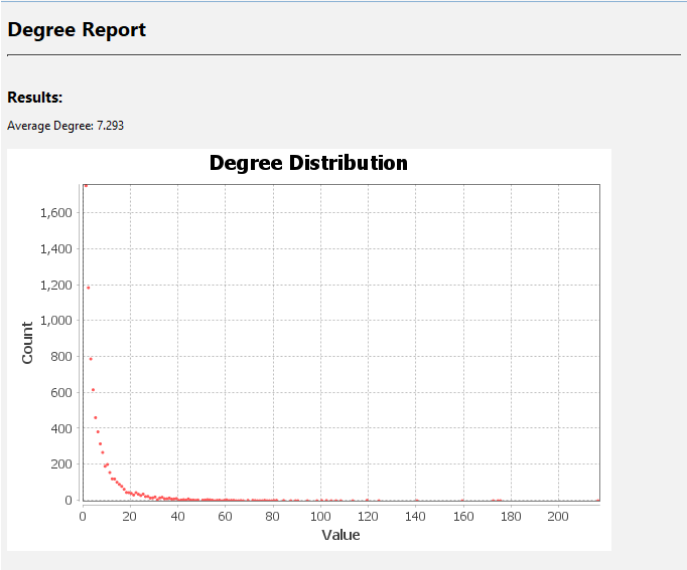
\includegraphics[width=0.7\textwidth]{s6p1.png}
\caption{Statistics -- average degree.}
\end{figure}

\newpage

\begin{figure}[!h]
\centering
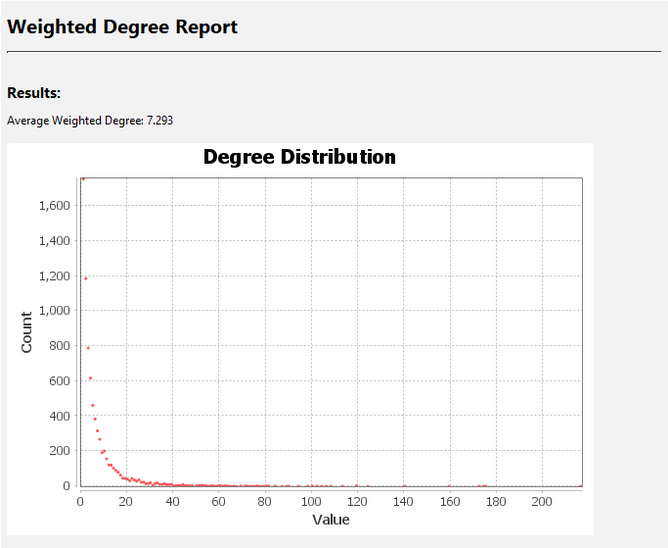
\includegraphics[width=0.65\textwidth]{s6p2.png}
\caption{Statistics -- average weighted degree.}
\end{figure}

\begin{figure}[!h]
\centering
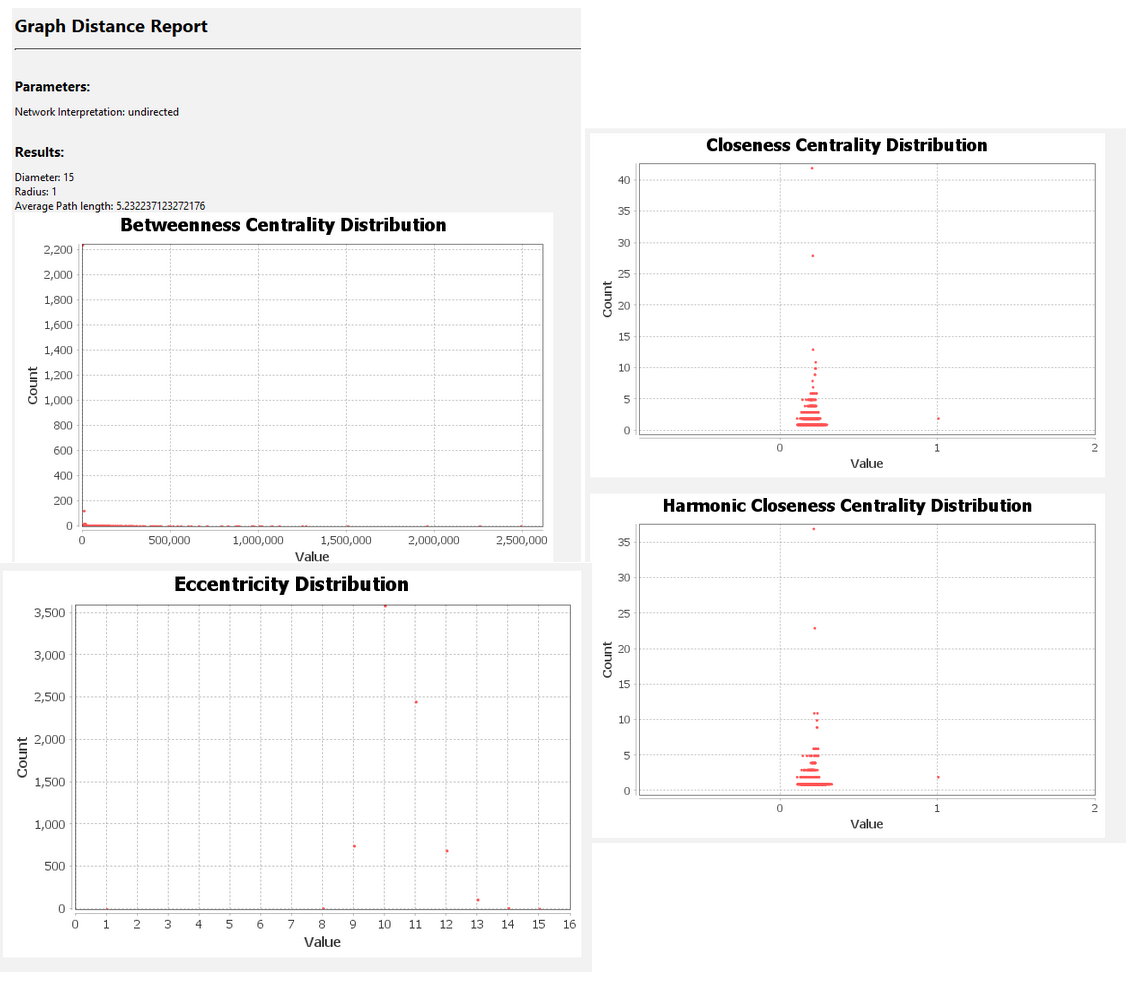
\includegraphics[width=0.9\textwidth]{s6p3.png}
\caption{Statistics -- network diameter.}
\end{figure}

\newpage

\textit{Graph density} measures how close the network is to complete. A complete graph has all possible edges and density equal to 1.
\begin{figure}[!h]
\centering
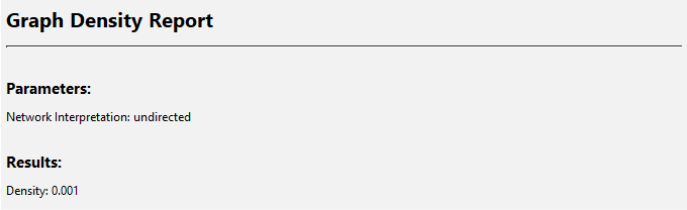
\includegraphics[width=0.65\textwidth]{s6p4.png}
\caption{Statistics -- graph density.}
\end{figure}

\textit{HITS} computes two separate values for each node. The first value (called Authority) measures how valuable information stored at that node is. The second value (called Hub) measures the quality of the nodes links.
\begin{figure}[!h]
\centering
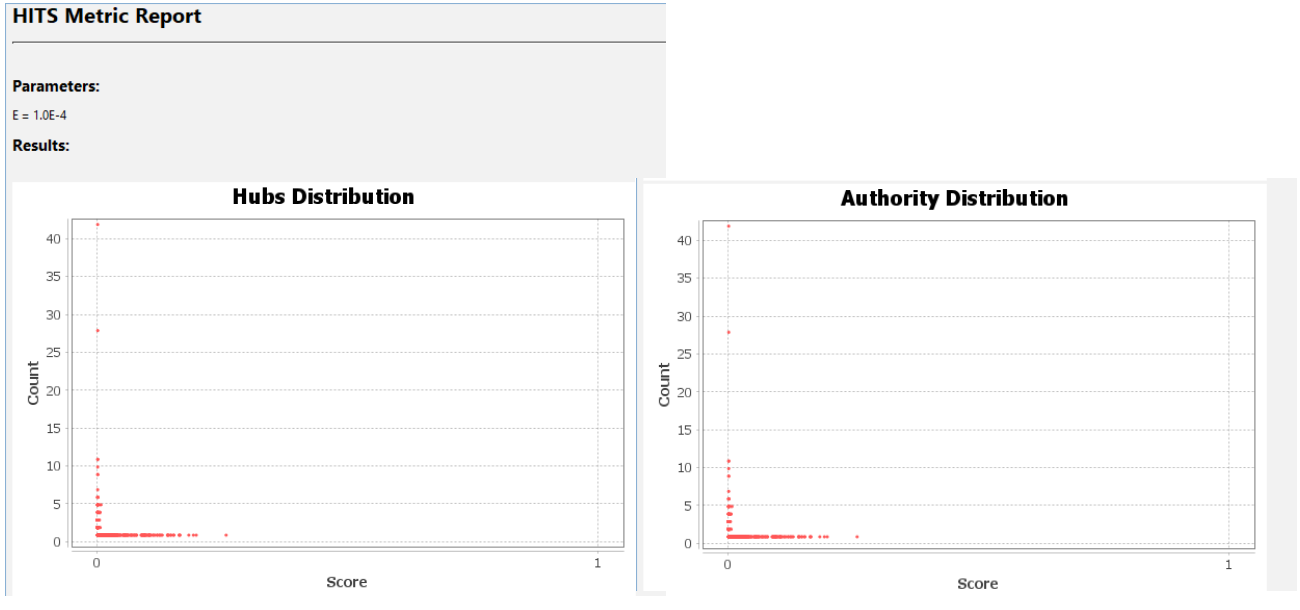
\includegraphics[width=0.95\textwidth]{s6p5.png}
\caption{Statistics -- HITS.}
\end{figure}

\newpage

\textit{PageRank} ranks nodes "pages" according to how often a user following links will non-randomly reach the node "page".
\begin{figure}[!h]
\centering
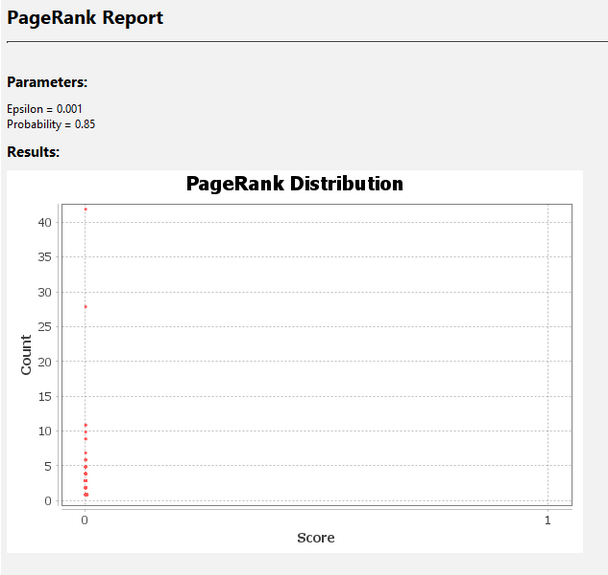
\includegraphics[width=0.55\textwidth]{s6p6.png}
\caption{Statistics -- PageRank.}
\end{figure}

\textit{Connected Components} determines the number of connected components in the network. For undirected graph detects only weakly connected components.
\begin{figure}[!h]
\centering
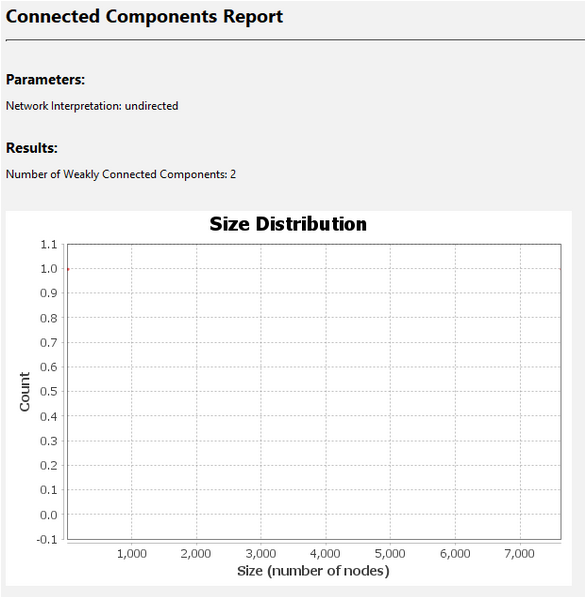
\includegraphics[width=0.55\textwidth]{s6p7.png}
\caption{Statistics -- connected components.}
\end{figure}

\newpage

\textit{Modularity} is a community detection algorithm.
\begin{figure}[!h]
\centering
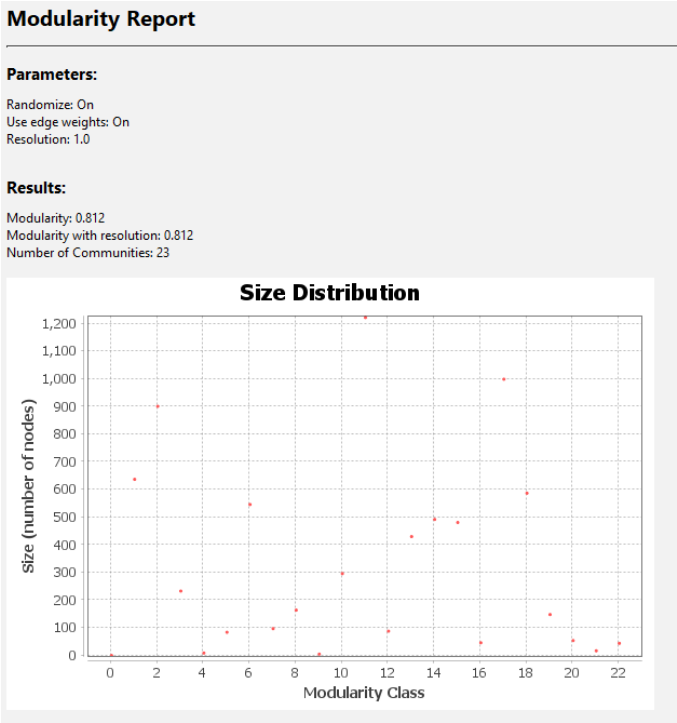
\includegraphics[width=0.65\textwidth]{s6p8.png}
\caption{Statistics -- modularity.}
\end{figure}

\begin{figure}[!h]
\centering
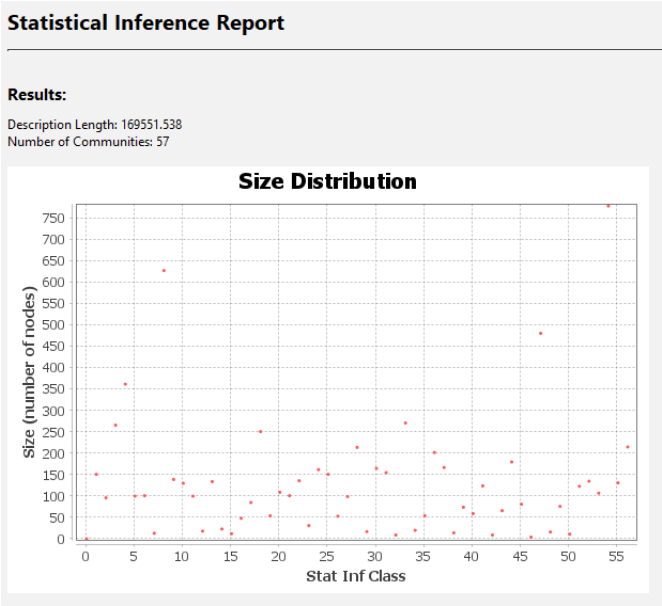
\includegraphics[width=0.65\textwidth]{s6p9.png}
\caption{Statistics -- statistical inference.}
\end{figure}

\newpage

The \textit{Average Clustering Coefficient}, along with the mean shortest path, can indicate a "small-world" effect. It indicates how nodes are embedded in their neighborhood. The average gives an overall indication of the clustering in the network. The Average Clustering Coefficient is the mean value of individual coefficients.
\begin{figure}[!h]
\centering
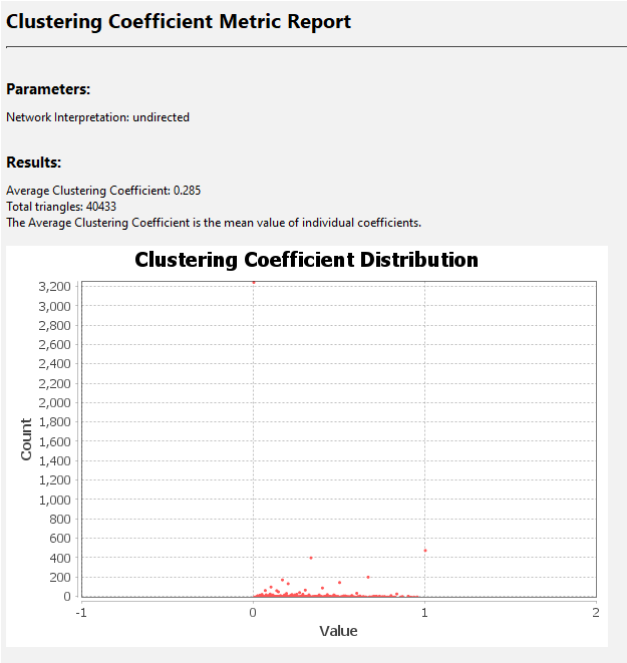
\includegraphics[width=0.55\textwidth]{s6p10.png}
\caption{Statistics -- Average Clustering Coefficient.}
\end{figure}

\textit{Eigenvector Centrality} is a measure of node importance in a network based on node's connections.
\begin{figure}[!h]
\centering
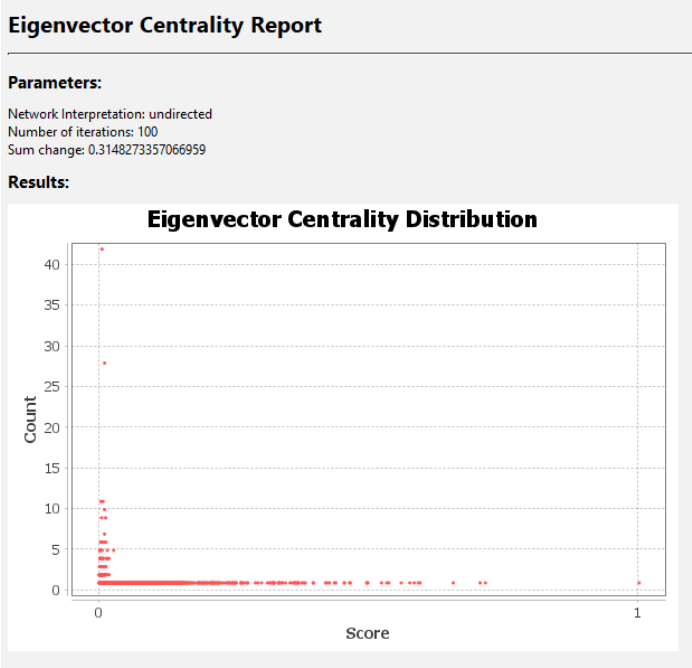
\includegraphics[width=0.55\textwidth]{s6p11.png}
\caption{Statistics -- Eigenvector Centrality.}
\end{figure}

\newpage

\textit{Network Diameter.} Distance is the average graph distance between all pairs of nodes. Connected nodes have graph distance 1. The diameter is the longest graph distance between any two nodes in the network. Related metrics:
\begin{itemize}
	\item \textit{Betweenness Centrality}: Measures how often a node appears on shortest paths between nodes in the network.
	\item \textit{Closeness Centrality}: The average distance from a given starting node to all other nodes in the network.
	\item \textit{Eccentricity}: The distance from a given starting node to the farthest node from it in the network.
\end{itemize}
\begin{figure}[!h]
\centering
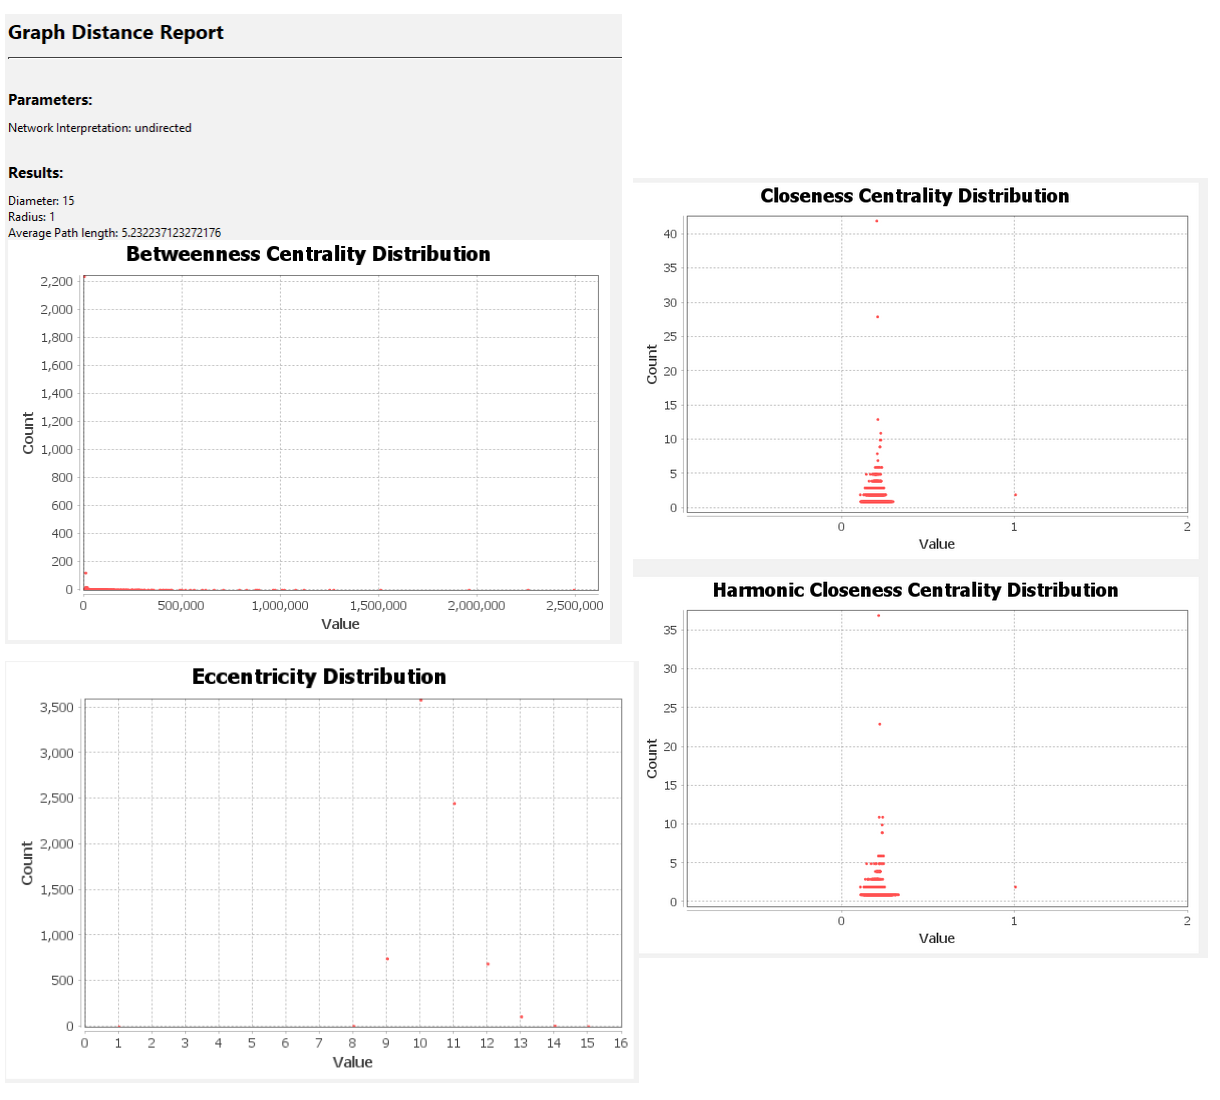
\includegraphics[width=\textwidth]{s6p12.png}
\caption{Statistics -- Network Diameter.}
\end{figure}

\newpage

\textbf{Step 7.} All network measures are summarized below.
\begin{figure}[!h]
\centering
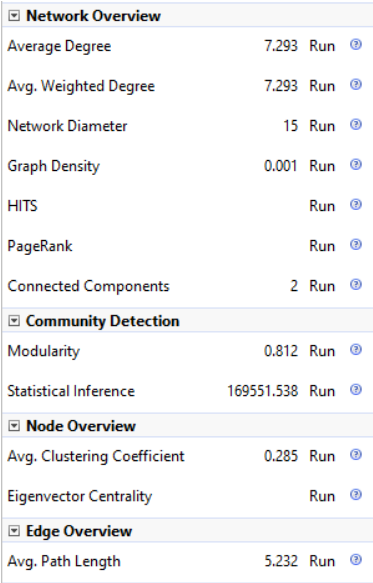
\includegraphics[width=0.45\textwidth]{s7p1.png}
\caption{All network measures.}
\end{figure}

Judging by the Density, the graph is incomplete. Average Degree and Average Weighted Degree are equal because the graph is unweighted.

\section*{Conclusions}
\addcontentsline{toc}{section}{Conclusions}

Gephi was used for analysis of a LastFM user network. It showed itself as a fast and optimized software package that lets user visualize large graphs and gather their metrics, both basic and complex.

\end{document}
